\documentclass[a4paper]{article}

\def\npart {IB}
\def\nterm {Lent}
\def\nyear {2016}
\def\nlecturer {A. G. Kovalev}
\def\ncourse {Geometry}
\def\nlectures {TT.10}
\def\nnotready {}

% Imports
\ifx \nextra \undefined
  \usepackage[pdftex,
    hidelinks,
    pdfauthor={Dexter Chua},
    pdfsubject={Cambridge Maths Notes: Part \npart\ - \ncourse},
    pdftitle={Part \npart\ - \ncourse},
  pdfkeywords={Cambridge Mathematics Maths Math \npart\ \nterm\ \nyear\ \ncourse}]{hyperref}
  \title{Part \npart\ - \ncourse}
\else
  \usepackage[pdftex,
    hidelinks,
    pdfauthor={Dexter Chua},
    pdfsubject={Cambridge Maths Notes: Part \npart\ - \ncourse\ (\nextra)},
    pdftitle={Part \npart\ - \ncourse\ (\nextra)},
  pdfkeywords={Cambridge Mathematics Maths Math \npart\ \nterm\ \nyear\ \ncourse\ \nextra}]{hyperref}

  \title{Part \npart\ - \ncourse \\ {\Large \nextra}}
\fi

\author{Lectured by \nlecturer \\\small Notes taken by Dexter Chua}
\date{\nterm\ \nyear}

\usepackage{alltt}
\usepackage{amsfonts}
\usepackage{amsmath}
\usepackage{amssymb}
\usepackage{amsthm}
\usepackage{booktabs}
\usepackage{caption}
\usepackage{enumitem}
\usepackage{fancyhdr}
\usepackage{graphicx}
\usepackage{mathtools}
\usepackage{microtype}
\usepackage{multirow}
\usepackage{pdflscape}
\usepackage{pgfplots}
\usepackage{siunitx}
\usepackage{tabularx}
\usepackage{tikz}
\usepackage{tkz-euclide}
\usepackage[normalem]{ulem}
\usepackage[all]{xy}

\pgfplotsset{compat=1.12}

\pagestyle{fancyplain}
\lhead{\emph{\nouppercase{\leftmark}}}
\ifx \nextra \undefined
  \rhead{
    \ifnum\thepage=1
    \else
      \npart\ \ncourse
    \fi}
\else
  \rhead{
    \ifnum\thepage=1
    \else
      \npart\ \ncourse\ (\nextra)
    \fi}
\fi
\usetikzlibrary{arrows}
\usetikzlibrary{decorations.markings}
\usetikzlibrary{decorations.pathmorphing}
\usetikzlibrary{positioning}
\usetikzlibrary{fadings}
\usetikzlibrary{intersections}
\usetikzlibrary{cd}

\newcommand*{\Cdot}{\raisebox{-0.25ex}{\scalebox{1.5}{$\cdot$}}}
\newcommand {\pd}[2][ ]{
  \ifx #1 { }
    \frac{\partial}{\partial #2}
  \else
    \frac{\partial^{#1}}{\partial #2^{#1}}
  \fi
}

% Theorems
\theoremstyle{definition}
\newtheorem*{aim}{Aim}
\newtheorem*{axiom}{Axiom}
\newtheorem*{claim}{Claim}
\newtheorem*{cor}{Corollary}
\newtheorem*{defi}{Definition}
\newtheorem*{eg}{Example}
\newtheorem*{fact}{Fact}
\newtheorem*{law}{Law}
\newtheorem*{lemma}{Lemma}
\newtheorem*{notation}{Notation}
\newtheorem*{prop}{Proposition}
\newtheorem*{thm}{Theorem}

\renewcommand{\labelitemi}{--}
\renewcommand{\labelitemii}{$\circ$}
\renewcommand{\labelenumi}{(\roman{*})}

\let\stdsection\section
\renewcommand\section{\newpage\stdsection}

% Strike through
\def\st{\bgroup \ULdepth=-.55ex \ULset}

% Maths symbols
\newcommand{\bra}{\langle}
\newcommand{\ket}{\rangle}

\newcommand{\N}{\mathbb{N}}
\newcommand{\Z}{\mathbb{Z}}
\newcommand{\Q}{\mathbb{Q}}
\renewcommand{\H}{\mathbb{H}}
\newcommand{\R}{\mathbb{R}}
\newcommand{\C}{\mathbb{C}}
\newcommand{\Prob}{\mathbb{P}}
\renewcommand{\P}{\mathbb{P}}
\newcommand{\E}{\mathbb{E}}
\newcommand{\F}{\mathbb{F}}
\newcommand{\cU}{\mathcal{U}}
\newcommand{\RP}{\mathbb{RP}}
\newcommand{\CP}{\mathbb{CP}}

\newcommand{\ph}{\,\cdot\,}

\DeclareMathOperator{\sech}{sech}
\DeclareMathOperator{\cosech}{cosech}
\DeclareMathOperator{\cosec}{cosec}

\DeclareMathOperator{\covol}{covol}
\DeclareMathOperator{\vol}{vol}

\let\Im\relax
\let\Re\relax
\DeclareMathOperator{\Im}{Im}
\DeclareMathOperator{\Re}{Re}
\DeclareMathOperator{\im}{im}
\DeclareMathOperator{\image}{image}
\DeclareMathOperator{\Ann}{Ann}

\DeclareMathOperator*{\res}{res}
\DeclareMathOperator{\Res}{Res}
\DeclareMathOperator{\Ind}{Ind}

\DeclareMathOperator{\tr}{tr}
\DeclareMathOperator{\diag}{diag}
\DeclareMathOperator{\rank}{rank}
\DeclareMathOperator{\card}{card}
\DeclareMathOperator{\spn}{span}
\DeclareMathOperator{\adj}{adj}

\DeclareMathOperator{\erf}{erf}
\DeclareMathOperator{\erfc}{erfc}

\DeclareMathOperator{\ord}{ord}
\DeclareMathOperator{\Sym}{Sym}

\DeclareMathOperator{\sgn}{sgn}
\DeclareMathOperator{\orb}{orb}
\DeclareMathOperator{\stab}{stab}
\DeclareMathOperator{\ccl}{ccl}

\DeclareMathOperator{\lcm}{lcm}
\DeclareMathOperator{\hcf}{hcf}

\DeclareMathOperator{\Int}{Int}
\DeclareMathOperator{\id}{id}

\DeclareMathOperator{\betaD}{beta}
\DeclareMathOperator{\gammaD}{gamma}
\DeclareMathOperator{\Poisson}{Poisson}
\DeclareMathOperator{\binomial}{binomial}
\DeclareMathOperator{\multinomial}{multinomial}
\DeclareMathOperator{\Bernoulli}{Bernoulli}
\DeclareMathOperator{\like}{like}

\DeclareMathOperator{\var}{var}
\DeclareMathOperator{\cov}{cov}
\DeclareMathOperator{\bias}{bias}
\DeclareMathOperator{\mse}{mse}
\DeclareMathOperator{\corr}{corr}

\DeclareMathOperator{\otp}{otp}
\DeclareMathOperator{\dom}{dom}

\DeclareMathOperator{\Root}{Root}
\DeclareMathOperator{\supp}{supp}
\DeclareMathOperator{\rel}{rel}
\DeclareMathOperator{\Hom}{Hom}
\DeclareMathOperator{\Aut}{Aut}
\DeclareMathOperator{\Gal}{Gal}
\DeclareMathOperator{\Mat}{Mat}
\DeclareMathOperator{\End}{End}
\DeclareMathOperator{\Char}{char}
\DeclareMathOperator{\ev}{ev}
\DeclareMathOperator{\St}{St}
\DeclareMathOperator{\Lk}{Lk}
\DeclareMathOperator{\disc}{disc}
\DeclareMathOperator{\Isom}{Isom}
\DeclareMathOperator{\length}{length}
\DeclareMathOperator{\energy}{energy}
\DeclareMathOperator{\area}{area}
\DeclareMathOperator{\Syl}{Syl}
\DeclareMathOperator{\cl}{cl}
\DeclareMathOperator{\fix}{fix}

\newcommand{\GL}{\mathrm{GL}}
\newcommand{\SL}{\mathrm{SL}}
\newcommand{\PGL}{\mathrm{PGL}}
\newcommand{\PSL}{\mathrm{PSL}}
\newcommand{\PSU}{\mathrm{PSU}}
\newcommand{\Or}{\mathrm{O}}
\newcommand{\SO}{\mathrm{SO}}
\newcommand{\U}{\mathrm{U}}
\newcommand{\SU}{\mathrm{SU}}

\renewcommand{\d}{\mathrm{d}}
\newcommand{\D}{\mathrm{D}}

\tikzset{->/.style = {decoration={markings,
                                  mark=at position 1 with {\arrow[scale=2]{latex'}}},
                      postaction={decorate}}}
\tikzset{<-/.style = {decoration={markings,
                                  mark=at position 0 with {\arrowreversed[scale=2]{latex'}}},
                      postaction={decorate}}}
\tikzset{<->/.style = {decoration={markings,
                                   mark=at position 0 with {\arrowreversed[scale=2]{latex'}},
                                   mark=at position 1 with {\arrow[scale=2]{latex'}}},
                       postaction={decorate}}}
\tikzset{->-/.style = {decoration={markings,
                                   mark=at position #1 with {\arrow[scale=2]{latex'}}},
                       postaction={decorate}}}
\tikzset{-<-/.style = {decoration={markings,
                                   mark=at position #1 with {\arrowreversed[scale=2]{latex'}}},
                       postaction={decorate}}}

\tikzset{circ/.style = {fill, circle, inner sep = 0, minimum size = 3}}
\tikzset{mstate/.style={circle, draw, blue, text=black, minimum width=0.7cm}}

\definecolor{mblue}{rgb}{0.2, 0.3, 0.8}
\definecolor{morange}{rgb}{1, 0.5, 0}
\definecolor{mgreen}{rgb}{0.1, 0.4, 0.2}
\definecolor{mred}{rgb}{0.5, 0, 0}

\def\drawcirculararc(#1,#2)(#3,#4)(#5,#6){%
    \pgfmathsetmacro\cA{(#1*#1+#2*#2-#3*#3-#4*#4)/2}%
    \pgfmathsetmacro\cB{(#1*#1+#2*#2-#5*#5-#6*#6)/2}%
    \pgfmathsetmacro\cy{(\cB*(#1-#3)-\cA*(#1-#5))/%
                        ((#2-#6)*(#1-#3)-(#2-#4)*(#1-#5))}%
    \pgfmathsetmacro\cx{(\cA-\cy*(#2-#4))/(#1-#3)}%
    \pgfmathsetmacro\cr{sqrt((#1-\cx)*(#1-\cx)+(#2-\cy)*(#2-\cy))}%
    \pgfmathsetmacro\cA{atan2(#2-\cy,#1-\cx)}%
    \pgfmathsetmacro\cB{atan2(#6-\cy,#5-\cx)}%
    \pgfmathparse{\cB<\cA}%
    \ifnum\pgfmathresult=1
        \pgfmathsetmacro\cB{\cB+360}%
    \fi
    \draw (#1,#2) arc (\cA:\cB:\cr);%
}
\newcommand\getCoord[3]{\newdimen{#1}\newdimen{#2}\pgfextractx{#1}{\pgfpointanchor{#3}{center}}\pgfextracty{#2}{\pgfpointanchor{#3}{center}}}

\def\Xint#1{\mathchoice
   {\XXint\displaystyle\textstyle{#1}}%
   {\XXint\textstyle\scriptstyle{#1}}%
   {\XXint\scriptstyle\scriptscriptstyle{#1}}%
   {\XXint\scriptscriptstyle\scriptscriptstyle{#1}}%
   \!\int}
\def\XXint#1#2#3{{\setbox0=\hbox{$#1{#2#3}{\int}$}
     \vcenter{\hbox{$#2#3$}}\kern-.5\wd0}}
\def\ddashint{\Xint=}
\def\dashint{\Xint-}


\begin{document}
\maketitle
{\small
\noindent Groups of rigid motions of Euclidean space. Rotation and reflection groups in two and three dimensions. Lengths of curves.\hspace*{\fill} [2]

\vspace{5pt}
\noindent Spherical geometry: spherical lines, spherical triangles and the Gauss-Bonnet theorem. Stereographic projection and M\"obius transformations.\hspace*{\fill} [3]

\vspace{5pt}
\noindent Triangulations of the sphere and the torus, Euler number.\hspace*{\fill} [1]

\vspace{5pt}
\noindent Riemannian metrics on open subsets of the plane. The hyperbolic plane. Poincar\'e models and their metrics. The isometry group. Hyperbolic triangles and the Gauss-Bonnet theorem. The hyperboloid model.\hspace*{\fill} [4]

\vspace{5pt}
\noindent Embedded surfaces in $\R^3$. The first fundamental form. Length and area. Examples.\hspace*{\fill} [1]

\vspace{5pt}
\noindent Length and energy. Geodesics for general Riemannian metrics as stationary points of the energy. First variation of the energy and geodesics as solutions of the corresponding Euler-Lagrange equations. Geodesic polar coordinates (informal proof of existence). Surfaces of revolution.\hspace*{\fill} [2]

\vspace{5pt}
\noindent The second fundamental form and Gaussian curvature. For metrics of the form $du^2 + G(u, v) dv^2$, expression of the curvature as $\sqrt{G_{uu}}/\sqrt{G}$. Abstract smooth surfaces and isometries. Euler numbers and statement of Gauss-Bonnet theorem, examples and applications.\hspace*{\fill} [3]}

\tableofcontents
\section{Euclidean geometry}
We are first going to look at Euclidean geometry. Roughly, this is the geometry of $\R^n$ under the usual inner product and norm.

\begin{defi}[(Standard) inner product]
  The \emph{(standard) inner product} on $\R^n$ is defined by
  \[
    (\mathbf{x}, \mathbf{y}) = \mathbf{x}\cdot \mathbf{y} = \sum_{i = 1}^n x_i y_i.
  \]
\end{defi}

\begin{defi}[Euclidean Norm]
  The \emph{Euclidean norm} of $\mathbf{x} \in \R^n$ is
  \[
    \|\mathbf{x}\| = \sqrt{(\mathbf{x}, \mathbf{x})}.
  \]
  This defines a metric on $\R^n$ by
  \[
    d(\mathbf{x}, \mathbf{y}) = \|\mathbf{x} - \mathbf{y}\|.
  \]
\end{defi}

\begin{defi}[Isometry]
  A map $f: \R^n \to \R^n$ is an \emph{isometry} of $\R^n$ if
  \[
    d(f(\mathbf{x}), f(\mathbf{y})) = d(\mathbf{x}, \mathbf{y})
  \]
  for all $\mathbf{x}, \mathbf{y} \in \R^n$.
\end{defi}
Note that $f$ is not required to be linear.

We would like to see some examples of isometries. A good source of examples is matrices. Recall the following definition:
\begin{defi}[Orthogonal matrix]
  An $n \times n$ matrix $A$ is \emph{orthogonal} if $AA^T = A^T A = I$.
\end{defi}

In general, for any matrix $A$ and $\mathbf{x}, \mathbf{y} \in \R^n$, we get
\[
  (A\mathbf{x}, A \mathbf{y}) = (A\mathbf{x})^T (A \mathbf{y}) = \mathbf{x}^T A^T A \mathbf{y} = (\mathbf{x}, A^T A \mathbf{y}).
\]
So $A$ is orthogonal if and only if $(A\mathbf{x}, A\mathbf{y}) = (\mathbf{x}, \mathbf{y})$ for all $\mathbf{x}, \mathbf{y} \in \R^n$.

Recall also that the inner product can be expressed in terms of the norm by
\[
  (\mathbf{x}, \mathbf{y}) = \frac{1}{2}(\|\mathbf{x} + \mathbf{y}\|^2 - \|\mathbf{x}\|^2 -\|\mathbf{y}\|^2).
\]
So if $A$ preserves in norm, then it preserves the inner product, and the converse is obviously true. So $A$ is orthogonal if and only if $\|A\mathbf{x}\| = \|\mathbf{x}\|$ for all $\mathbf{x} \in \R^n$. Hence matrices are orthogonal if and only if they are isometries.

More generally, let
\[
  f(\mathbf{x}) = A\mathbf{x} + \mathbf{b}.
\]
Then
\[
  d(f(\mathbf{x}), f(\mathbf{y})) = \|A(\mathbf{x} - \mathbf{y})\|.
\]
So any $f$ of this form is an isometry if and only if $A$ is orthogonal. This is not too surprising. What might not be expected is that all isometries are of this form.

\begin{thm}
  Every isometry of $f: \R^n \to \R^n$ is of the form
  \[
    f(\mathbf{x}) = A\mathbf{x} + \mathbf{b}.
  \]
  for $A$ orthogonal and $\mathbf{b} \in \R^n$.
\end{thm}

\begin{proof}
  Let $f$ be an isometry. Let $\mathbf{e}_1, \cdots, \mathbf{e}_n$ be the standard basis of $\R^n$. Let
  \[
    \mathbf{b} = f(\mathbf{0}), \quad \mathbf{a}_i = f(\mathbf{e}_i) - \mathbf{b}.
  \]
  The idea is to construct our matrix $A$ out of these $\mathbf{a}_i$. For $A$ to be orthogonal, $\{\mathbf{a}_i\}$ must be an orthonormal basis.

  Indeed, we can compute
  \[
    \|\mathbf{a}_i\| = \|\mathbf{f}(\mathbf{e}_i) - f(\mathbf{0})\| = d(f(\mathbf{e}_i), f(\mathbf{0})) = d(\mathbf{e}_i, \mathbf{0}) = \|\mathbf{e}_i\| = 1.
  \]
  For $i \not = j$, we have
  \begin{align*}
    (\mathbf{a}_i, \mathbf{a}_j) &= -(\mathbf{a}_i, -\mathbf{a}_j) \\
    &=-\frac{1}{2}(\|\mathbf{a}_i - \mathbf{a}_j\|^2 - \|\mathbf{a}_i\|^2 - \mathbf{a}_j\|^2)\\
    &= -\frac{1}{2}(\|f(\mathbf{e}_i) - f(\mathbf{e}_j)\|^2 - 2)\\
    &= -\frac{1}{2}(\|\mathbf{e}_i - \mathbf{e}_j\|^2 - 2)\\
    &= 0
  \end{align*}
  So $\mathbf{a}_i$ and $\mathbf{a}_j$ are orthogonal. In other words, $\{\mathbf{a}_i\}$ forms an orthonormal set. It is an easy result that any orthogonal set must be linearly independent. Since we have found $n$ orthonormal vectors, they form an orthonormal basis.

  Hence, the matrix $A$ with columns given by the column vectors $\mathbf{a}_i$ is an orthogonal matrix. We define a new isometry
  \[
    g(\mathbf{x}) = A\mathbf{x} + \mathbf{b}.
  \]
  We want to show $f = g$. By construction, we know $g(\mathbf{x}) = f(\mathbf{x})$ is true for $\mathbf{x} = \mathbf{0}, \mathbf{e}_1, \cdots, \mathbf{e}_n$.

  We observe that $g$ is invertible. In particular,
  \[
    g^{-1}(\mathbf{x}) = A^{-1}(\mathbf{x} - \mathbf{b}) = A^T \mathbf{x} - A^T\mathbf{b}.
  \]
  Moreover, it is an isometry.

  We define
  \[
    h = g^{-1}\circ f.
  \]
  Since it is a composition of isometries, it is also an isometry. Moreover, it fixes $\mathbf{x} = \mathbf{0}, \mathbf{e}_1, \cdots, \mathbf{e}_n$.

  It currently suffices to prove that $h$ is the identity.

  Let $\mathbf{x} \in \R^n$, and expand it in the basis as
  \[
    \mathbf{x} = \sum_{i = 1}^n x_i \mathbf{e}_i.
  \]
  Let
  \[
    \mathbf{y} = h(\mathbf{x}) = \sum_{i = 1}^n y_i \mathbf{e}_i.
  \]
  We can compute
  \begin{align*}
    d(\mathbf{x}, \mathbf{e}_i)^2 &= (\mathbf{x} - \mathbf{e}_i, \mathbf{x} - \mathbf{e}_i) = \|\mathbf{x}\|^2 + 1 - 2 x_i\\
    d(\mathbf{x}, 0)^2 &= \|\mathbf{x}\|^2.
  \end{align*}
  Similarly, we have
  \begin{align*}
    d(\mathbf{y}, \mathbf{e}_i)^2 &= (\mathbf{y} - \mathbf{e}_i, \mathbf{y} - \mathbf{e}_i) = \|\mathbf{y}\|^2 + 1 - 2 y_i\\
    d(\mathbf{y}, 0)^2 &= \|\mathbf{y}\|^2.
  \end{align*}
  Since $h$ is an isometry and fixes $\mathbf{0}, \mathbf{e}_1, \cdots, \mathbf{e}_n$, and by definition $h(\mathbf{x}) = \mathbf{y}$, we must have
  \[
    d(\mathbf{x}, \mathbf{0}) = d(\mathbf{y}, \mathbf{0}), \quad d(\mathbf{x}, \mathbf{e}_i) = d(\mathbf{y}, \mathbf{e}_i).
  \]
  These give $\|\mathbf{x}\|^2 = \|\mathbf{y}\|^2$, and hence $x_i = y_i$ for all $i$. In other words, $\mathbf{x} = \mathbf{y} = h(\mathbf{x})$. So $h$ is the identity.
\end{proof}

\begin{defi}[Isometry group]
  The \emph{isometry group} $\Isom(\R^n)$ is the group of all isometries of $\R^n$, which is a group by composition.
\end{defi}

\begin{eg}[Reflections in an affine hyperplane]
  Let $H \subseteq \R^n$ be an affine hyperplane given by
  \[
    H = \{\mathbf{x} \in \R^n: \mathbf{u} \cdot \mathbf{x} = c\},
  \]
  where $\|\mathbf{u}\| = 1$ and $c \in \R$. This is just a natural generalization of a 2-dimensional plane in $\R^3$. Note that unlike a vector subspace, it does not have to contain the origin.

  Reflection in $H$, written $R_H$, is the map
  \begin{align*}
    R_H: \R^n &\to \R^n\\
    \mathbf{x} &\mapsto \mathbf{x} - 2(\mathbf{x} \cdot \mathbf{u} - c)\mathbf{u}
  \end{align*}
  It is an exercise in the example sheet to show that this is indeed an isometry.

  We now check this is indeed what we think a reflection should be. Note that every point in $\R^n$ can be written as $\mathbf{a} + t\mathbf{u}$, where $\mathbf{a} \in H$. Then the reflection should send this point to $\mathbf{a} - t\mathbf{u}$.
  \begin{center}
    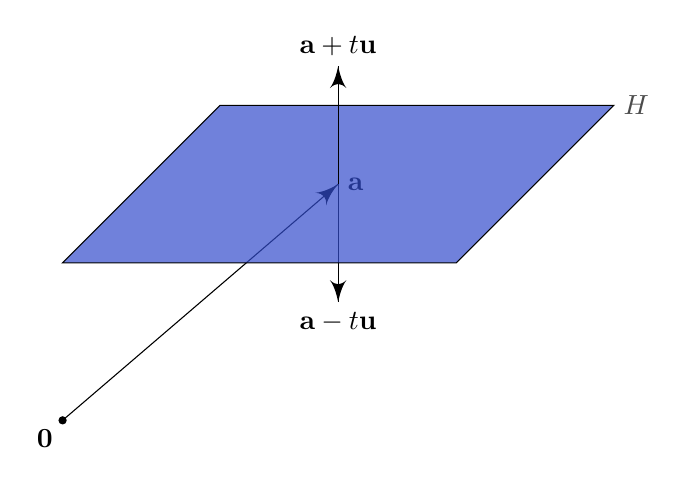
\begin{tikzpicture}
      \node [circ] at (0, -2) {};
      \node [anchor = north east] at (0, -2) {$\mathbf{0}$};
      \draw [->] (0, -2) -- (3.5, 1) node [right] {$\mathbf{a}$};
      \draw [->] (3.5, 1) -- +(0, -1.5) node [below] {$\mathbf{a} - t\mathbf{u}$};
      \draw [fill=mblue, fill opacity=0.7] (0, 0) -- (5, 0) -- (7, 2) node [right] {$H$} -- (2, 2) -- cycle;
      \draw [->] (3.5, 1) -- +(0, 1.5) node [above] {$\mathbf{a} + t\mathbf{u}$};
    \end{tikzpicture}
  \end{center}
  This is a routine check:
  \[
    R_H (\mathbf{a} + t\mathbf{u}) = (\mathbf{a} + t\mathbf{u}) - 2t\mathbf{u} = \mathbf{a} - t\mathbf{u}.
  \]
  In particular, we know $R_H$ fixes exactly the points of $H$.

  The converse is also true --- any isometry $S \in \Isom(\R^n)$ that fixes the points in some affine hyperplane $H$ is either the identity or $R_H$.

  First, we want to translate the plane such that it becomes a vector subspace. Then we can use our linear algebra magic. For any $\mathbf{a} \in \R^n$, we can define the translation by $\mathbf{a}$ as
  \[
    T_{\mathbf{a}}(\mathbf{x}) = \mathbf{x} + \mathbf{a}.
  \]
  This is clearly an isometry.

  We pick an arbitrary $\mathbf{a} \in H$, and let $R = T_{-\mathbf{a}} S T_\mathbf{a} \in \Isom(\R^n)$. Then $R$ fixes exactly $H' = T_{-\mathbf{a}} H$. Since $\mathbf{0} \in H'$, $H'$ is a vector subspace. In particular, if $H = \{\mathbf{x}: \mathbf{x}\cdot \mathbf{u} = c\}$, then by putting $c = \mathbf{a}\cdot \mathbf{u}$, we find
  \[
    H' = \{\mathbf{x}: \mathbf{x}\cdot \mathbf{u} = 0\}.
  \]
  To understand $R$, we already know it fixes everything in $H'$. So we want to see what it does to $\mathbf{u}$. Note that since $R$ is an isometry and fixes the origin, it is in fact an orthogonal map. Hence for any $\mathbf{x} \in H'$, we get
  \[
    (R\mathbf{u}, \mathbf{x}) = (R\mathbf{u}, R\mathbf{x}) = (\mathbf{u}, \mathbf{x}) = 0.
  \]
  So $R\mathbf{u}$ is also perpendicular to $H'$. Hence $R\mathbf{u} = \lambda \mathbf{u}$ for some $\lambda$. Since $R$ is an isometry, we have $\|R\mathbf{u}\|^2 = 1$. Hence $|\lambda|^2 = 1$, and thus $\lambda = \pm 1$. So either $\lambda = 1$, and $R = \id$; or $\lambda = -1$, and $R = R_{H'}$, as we already know for orthogonal matrices.

  It thus follow that $S = \id_{\R^n}$, or $S$ is a reflection, as we will show in the next lecture.
\end{eg}
\end{document}
